\documentclass[10pt,xcolor={rgb}]{beamer}
    
    \usetheme{metropolis}
    \usepackage[utf8]{inputenc}
    
    \usepackage{appendixnumberbeamer}
    
    \usepackage{booktabs}
    \usepackage[scale=2]{ccicons}
    
    \usepackage{pgfplots}
    \usepgfplotslibrary{dateplot}
    
    \usepackage{xspace}
    \newcommand{\themename}{\textbf{\textsc{metropolis}}\xspace}

    \usepackage{smartdiagram}
    \usesmartdiagramlibrary{additions}

    \usepackage{tikz}
    \usetikzlibrary{arrows,decorations.pathmorphing,backgrounds,fit,positioning,shapes.symbols,chains, shapes.arrows}

    \definecolor{bluei}{RGB}{83,116,191}
    \definecolor{blueii}{RGB}{207,212,232}
    \definecolor{greeni}{RGB}{135,200,81}
    \definecolor{greenii}{RGB}{216,235,207}
    \definecolor{grayi}{RGB}{160,160,160}

    \tikzset{
      myiblock/.style 2 args={
        draw=white,
        fill=#1,
        line width=1pt,
        rounded corners,
        align=center,
        text=white,
        font=\sffamily,
        text width=#2,
        minimum height=1cm
      },
      myoblock/.style={
        fill=#1,
        rounded corners,
        align=center,
        inner xsep=10pt
      },
      myserverblock/.style={
        fill=#1,
        rounded corners,
        align=center,
        inner xsep=15pt,
        inner ysep=6pt,
        draw=white,
      },
      myminiblock/.style 2 args={
        draw=white,
        fill=#1,
        line width=1pt,
        rounded corners,
        align=center,
        text=white,
        font=\sffamily,
        text width=#2,
        minimum height=0.5cm,
      },
    }

    \usepackage{graphicx}
    \graphicspath{ {img/} }


    \title{Control de versions}
    \subtitle{Introducció als sistemes de gestió de canvis}
    \date{28/09/2017}
    \author{Josep Maria Pinyol Fontseca}
    \institute{Endepro Software, S.L.}
    % \titlegraphic{\hfill\includegraphics[height=1.5cm]{logo.pdf}}

    \begin{document}

    \maketitle
    
    \begin{frame}{Continguts}
      \setbeamertemplate{section in toc}[sections numbered]
      \tableofcontents[hideallsubsections]
    \end{frame}
    
    
    \section{Introducció}    
    
    \begin{frame}[fragile]{Presentació}

      \begin{block}{Qui sóc?}

        Em dic \textbf{Josep Maria Pinyol Fontseca} i porto 20 anys a la indústria del software des de desenvolupador fins a director de projectes.

        \begin{itemize}
          \item Treballant amb control de versions des del 1998
          \item Realització i participació de projectes petits fins a grans projectes amb desenes de desenvolupadors
          \item A \textbf{Endepro Software} des de fa 14 anys
        \end{itemize}

        \centering
        
\includegraphics[width=2cm, height=2cm]{endepro.png}
      \end{block}

    \end{frame}


    \begin{frame}[fragile]{Introducció}

      \begin{block}{Qué és un sistema de control de versions?}
        \begin{itemize}
          \item Gestió de canvis d'arxius en el temps
          \item Revertir un arxiu a una versió anterior de forma simple
          \item Comparar canvis en el temps
          \item Visualitzar qui ha realitzat determinats canvis en un fitxer
          \item S'utilitza principalment a la industria informàtica
        \end{itemize}
      \end{block}
      
    \end{frame}

    \section{Sistemes de control de versions}
    
    \begin{frame}[fragile]{Sistema de control habitural}

      Un dels primers sistemes de control de versions els coneixem perfectament. 
      \begin{block}{Segurament molts de nosaltres hem fet això més d'una vegada:}
      \begin{itemize}
        \item Oferta.docx
        \item Oferta-Copia.docx
        \item Oferta-Copia (2).docx
        \item Oferta-BO.docx
        \item Oferta-BO-2.docx
      \end{itemize}
      \end{block}
      I quina és l'oferta bona?
    \end{frame}

    \begin{frame}[fragile]{Sistema de control habitural}
      
      \begin{block}{Si sóm molt organitzats inclourem la data i hora en el nom del fitxer:}
            
            \begin{itemize}
              \item Oferta-18-6-2017-17:20.docx
              \item Oferta-18-6-2017-17:25.docx
              \item Oferta-19-6-2017-8:42.docx
              \item Oferta-19-6-2017-9:15.docx
            \end{itemize}

      \end{block}
      El mateix pasa amb projectes sencers que estan en una carpeta, fent versions de les carpetes, etc.
    \end{frame}
          
    \begin{frame}[fragile]{Per què necessitem un sistema de control de versions?}
      
      \begin{block}{Però, per què realment necessitem un sistema de control de versions:}
            
            \begin{itemize}
              \item Còpia i restauració:  podem saltar a una versió del dia que vulguem
              \item Sincronització: podem compartir els fitxers i tenir la última versió
              \item Desfer a curt termini:  podem tirar enrera dels canvis que hem anat fent durant els últims dies
              \item Desfer a llarg termini:  si necessitem una versió de fa 1 any, cap problema
              \item Control de canvis:  controlar tots els canvis que es fan en els fitxers 
              \item Control dels usuaris:  tenim el nom i cognoms de qui ha fet el canvi
              \item Branques i unions:  si volem fer molts canvis en un projecte, podem aïllar el nostre codi, fer els canvis i unir-ho tot un cop estigui fet
            \end{itemize}

      \end{block}

    \end{frame}

    \begin{frame}[fragile]{Tipus de Sistemes de control de versions}
      
            
      \begin{block}{Evolució i generacions dels sistemes de control de versions:}
        
        \begin{enumerate}
          \item Sistemes de control de versions locals
          \item Sistemes de control de versions centralitzats
          \item Sistemes de control de versions distribuïts
        \end{enumerate}

      \end{block}

    \end{frame}
      
    \begin{frame}[fragile]{Sistemes de control de versions locals}
      
      \begin{block}{Primera generació: local}
        
        \begin{itemize}
          \item Disponible per a sistemes UNIX des del 1972
          \item Disenyat per controlar els canvis realitats en el codi font o fitxers de text
          \item Tenim disponible el RCS per vàries plataformes
        \end{itemize}

      \end{block}

      \begin{center}
        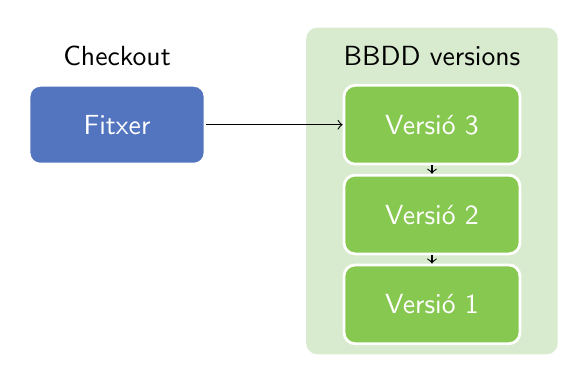
\begin{tikzpicture}[node distance=0.5cm and 1cm]
          \node[myiblock={bluei}{2cm}]
            (info1)
            {Fitxer};
          \node[above=3pt of info1,font=\sffamily]
            (title1)
            {Checkout};

          \begin{scope}[xshift=4cm,node distance=3pt and 1cm]
          \node[myiblock={greeni}{2cm}]
            (infoob1)
            {Versió 3};
          \node[myiblock={greeni}{2cm},below=of infoob1]
            (infoob2)
            {Versió 2};
          \node[myiblock={greeni}{2cm},below=of infoob2]
            (infoob3)
            {Versió 1};
          \node[above=3 pt of infoob1,font=\sffamily]
            (title2)
            {BBDD versions};
          \begin{pgfonlayer}{background}
          \node[myoblock=greenii,fit={(title2) (infoob3)}] {};  
          \end{pgfonlayer}
          \end{scope}

          \draw [->] (info1) edge (infoob1);
          \draw [->] (infoob1) edge (infoob2) (infoob2) edge (infoob3);
        \end{tikzpicture}
      \end{center}

    \end{frame}

    \begin{frame}[fragile]{Sistemes de control de versions centralitzat}

      \begin{block}{Segona generació: centralitzat}
        
        \begin{itemize}
          \item Disponible des del 1986
          \item Arquitectura client servidor
          \item Les implementacions més utilitzades són: CVS, Subversion (SVN)
        \end{itemize}

      \end{block}

      \begin{center}
        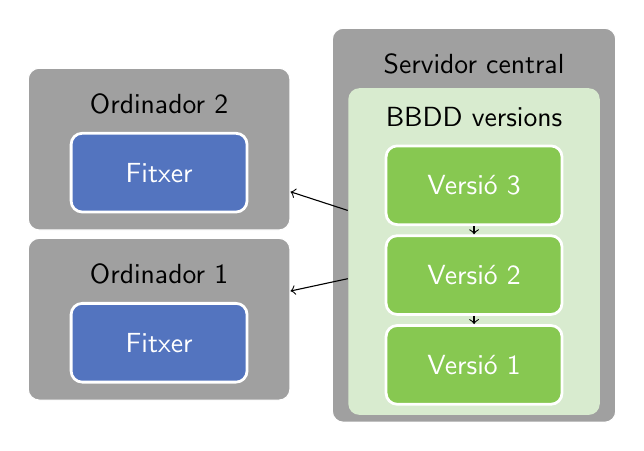
\begin{tikzpicture}[node distance=0.5cm and 1cm]

          \node[myiblock={bluei}{2cm}]
            (fitxer1)
            {Fitxer};
          \node[above=3pt of fitxer1,font=\sffamily]
            (ordinador1)
            {Ordinador 1};

          \node[above=15pt of ordinador1, myiblock={bluei}{2cm}]
            (fitxer2)
            {Fitxer};
          \node[above=3pt of fitxer2,font=\sffamily]
            (ordinador2)
            {Ordinador 2};

          \begin{pgfonlayer}{background}
            \node[myserverblock=grayi,fit={(fitxer2) (ordinador2)}] (repoord1) {};  
          \end{pgfonlayer}

          \begin{pgfonlayer}{background}
            \node[myserverblock=grayi,fit={(fitxer1) (ordinador1)}] (repoord2) {};  
          \end{pgfonlayer}

          \begin{scope}[yshift=2cm, xshift=4cm,node distance=3pt and 1cm]
          \node[myiblock={greeni}{2cm}]
            (infoob1)
            {Versió 3};
          \node[myiblock={greeni}{2cm},below=of infoob1]
            (infoob2)
            {Versió 2};
          \node[myiblock={greeni}{2cm},below=of infoob2]
            (infoob3)
            {Versió 1};
          \node[above=3 pt of infoob1,font=\sffamily]
            (title2)
            {BBDD versions};
          \node[above=5 pt of title2,font=\sffamily]
            (title3)
            {Servidor central};         
            
            \begin{pgfonlayer}{background}
              \node[myserverblock=grayi,fit={(title3) (infoob3)}] {};  
            \end{pgfonlayer}
            
          \begin{pgfonlayer}{background}
          \node[myoblock=greenii,fit={(title2) (infoob3)}] (repo) {};  
          \end{pgfonlayer}

          \end{scope}

          \draw [->] (repo) edge (repoord1);
          \draw [->] (repo) edge (repoord2);
          \draw [->] (infoob1) edge (infoob2) (infoob2) edge (infoob3);
        \end{tikzpicture}
      \end{center}
    
    
    \end{frame}

    \begin{frame}[fragile]{Sistemes de control distribuït}

      \begin{block}{Tercera generació: distribuït}
        
        \begin{itemize}
          \item Disponible des del 2000
          \item Arquitectura desentralitzada o distribuïda
          \item Les implementacions més utilitzades són: GIT, Mercurial (HG)
        \end{itemize}

        \begin{center}
          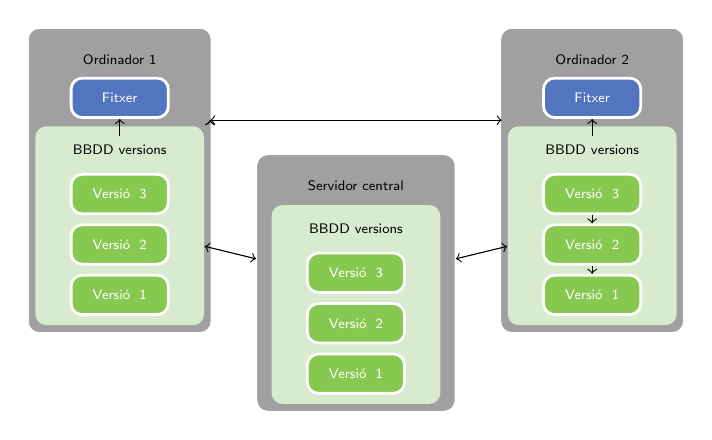
\begin{tikzpicture}[node distance=0.5cm and 1cm]

            %Servidor central
            \begin{scope}[xshift=4cm,node distance=3pt and 1cm]
            \node[myminiblock={greeni}{1cm}]
              (infoob1)
              {\tiny Versió 3};
            \node[myminiblock={greeni}{1cm},below=of infoob1]
              (infoob2)
              {\tiny Versió 2};
            \node[myminiblock={greeni}{1cm},below=of infoob2]
              (infoob3)
              {\tiny Versió 1};
            \node[above=3 pt of infoob1,font=\sffamily]
              (title2)
              {\tiny BBDD versions};

              \node[above=5 pt of title2,font=\sffamily]
              (title3)
              {\tiny Servidor central};         
              
              \begin{pgfonlayer}{background}
                \node[myserverblock=grayi,fit={(title3) (infoob3)}] (backServer) {};  
              \end{pgfonlayer}

              \begin{pgfonlayer}{background}
              \node[myoblock=greenii,fit={(title2) (infoob3)}] {};  
              \end{pgfonlayer}

            \end{scope}

            %Ordinador 1
            \begin{scope}[yshift=1cm,xshift=1cm,node distance=3pt and 1cm]
              \node[myminiblock={greeni}{1cm}]
                (infoob1)
                {\tiny Versió 3};
              \node[myminiblock={greeni}{1cm},below=of infoob1]
                (infoob2)
                {\tiny Versió 2};
              \node[myminiblock={greeni}{1cm},below=of infoob2]
                (infoob3)
                {\tiny Versió 1};
              \node[above=3 pt of infoob1,font=\sffamily]
                (title2Ordinador1)
                {\tiny BBDD versions};
  
                \node[myminiblock={bluei}{1cm}, above=6pt of title2Ordinador1]
                (fitxerOrdinador1)
                {\tiny Fitxer};    
  
                \node[above=1 pt of fitxerOrdinador1,font=\sffamily]
                (title3)
                {\tiny Ordinador 1};         
   
                
                \begin{pgfonlayer}{background}
                  \node[myserverblock=grayi,fit={(title3) (infoob3)}] {};  
                \end{pgfonlayer}
  
                \begin{pgfonlayer}{background}
                \node[myoblock=greenii,fit={(title2Ordinador1) (infoob3)}] (backOrdinador1) {};  
                \end{pgfonlayer}
  
            \end{scope}

            %Ordinador 2
            \begin{scope}[yshift=1cm,xshift=7cm,node distance=3pt and 1cm]
              \node[myminiblock={greeni}{1cm}]
                (infoob1)
                {\tiny Versió 3};
              \node[myminiblock={greeni}{1cm},below=of infoob1]
                (infoob2)
                {\tiny Versió 2};
              \node[myminiblock={greeni}{1cm},below=of infoob2]
                (infoob3)
                {\tiny Versió 1};
              \node[above=3 pt of infoob1,font=\sffamily]
                (title2Ordinador2)
                {\tiny BBDD versions};

                \node[myminiblock={bluei}{1cm}, above=6pt of title2Ordinador2]
                (fitxerOrdinador2)
                {\tiny Fitxer};    
  
                \node[above=1 pt of fitxerOrdinador2,font=\sffamily]
                (title3)
                {\tiny Ordinador 2};         
                
                \begin{pgfonlayer}{background}
                  \node[myserverblock=grayi,fit={(title3) (infoob3)}] {};  
                \end{pgfonlayer}
  
                \begin{pgfonlayer}{background}
                \node[myoblock=greenii,fit={(title2Ordinador2) (infoob3)}] (backOrdinador2) {};  
                \end{pgfonlayer}
  
            \end{scope}
  
            \draw [->] (infoob1) edge (infoob2) (infoob2) edge (infoob3);
            \draw [->] (title2Ordinador2) edge (fitxerOrdinador2);
            \draw [->] (title2Ordinador1) edge (fitxerOrdinador1);
            \draw [<->] ([yshift=2pt, xshift=2pt] backOrdinador1.north east) edge ([yshift=2pt, xshift=-2pt] backOrdinador2.north west);
            \draw [<->] (backOrdinador1) edge (backServer);
            \draw [<->] (backOrdinador2) edge (backServer);
            
          \end{tikzpicture}
        \end{center}

      \end{block}

    \end{frame}

    \begin{frame}[fragile]{Avantatges del sistema Distribuït vs Centralitzat}
      
            \begin{block}{Principals avantatges del sistema distribuït:}
      
              \begin{itemize}
                \item Tothom té una còpia local del codi
                \item Es pot treballar Offline
                \item És ràpid, tot es fa localment i no en el servidor central
                \item Els canvis es gestionen millor al tenir un GUID per canvi realitzat
                \item Les Branques i les Unions són fàcils ja que cada desenvolupador té la seva pròpia Branca
                \item Menys gestió, ja que no cal un servidor central en funcionament
              \end{itemize}
      
            \end{block}
      
    \end{frame}

    \begin{frame}[fragile]{Revisions}
      
            \begin{block}{Revisions}
      
              \begin{itemize}
                \item Cada cop que fem una nova versió tenim una nova revisió del fitxer
              \end{itemize}

              \centering
              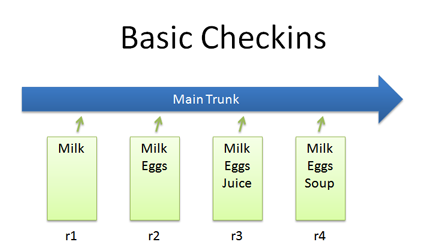
\includegraphics[height=4cm]{basic_checkin.png}
      
            \end{block}
      
    \end{frame}

    \begin{frame}[fragile]{Canvis i edició}
      
            \begin{block}{Canvis i edició}
      
              \begin{itemize}
                \item En realitat obtenir la revisió, editem i guardem la revisió
                \item Podem desfer els canvis a una revisió anterior sempre que vulguem
              \end{itemize}

              \centering
              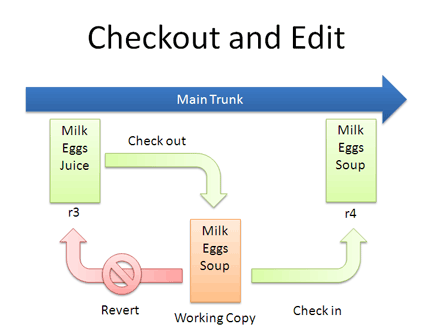
\includegraphics[height=4cm]{checkout_edit.png}
      
            \end{block}
      
    \end{frame}

    \begin{frame}[fragile]{Diferències}
      
            \begin{block}{Diferències}
      
              \begin{itemize}
                \item Es guarden les diferències entres revisions
                \item La majoria de sistemes de control de versions guarden aquests diferencies en comptes de tots els fitxers
              \end{itemize}

              \centering
              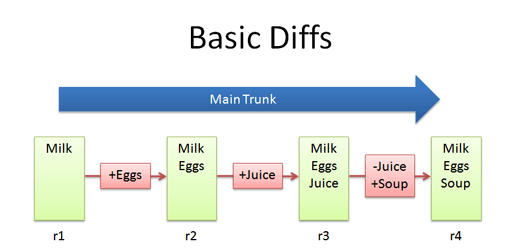
\includegraphics[height=4cm]{basic_diffs.png}
      
            \end{block}
      
    \end{frame}


    \begin{frame}[fragile]{Branques}
      
            \begin{block}{Branques}
      
              \begin{itemize}
                \item Les branques ens permeten fer una còpia del codi en una "carpeta" diferent
                
              \end{itemize}

              \centering
              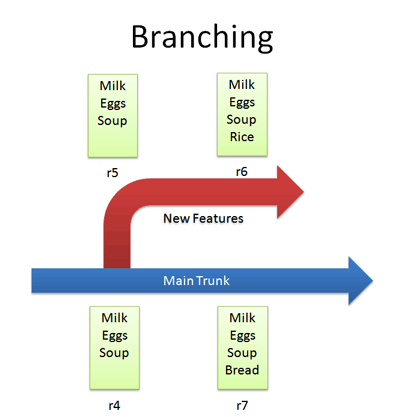
\includegraphics[height=6cm]{first_branch.png}
      
            \end{block}
      
    \end{frame}


    \begin{frame}[fragile]{Unions o Merge}
      
            \begin{block}{Merge}
      
              \begin{itemize}
                \item En permet unir canvis realitzats de branques diferents
                
              \end{itemize}

              \centering
              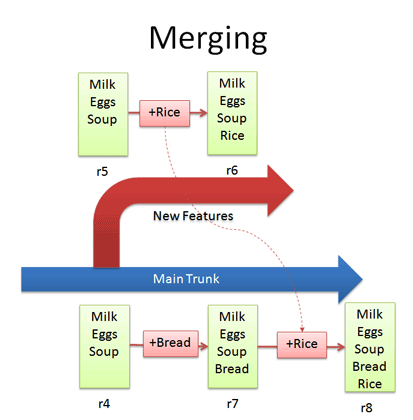
\includegraphics[height=6cm]{merging.png}
      
            \end{block}
      
    \end{frame}

    \begin{frame}[fragile]{Conflictes}
      
            \begin{block}{Conflictes}
      
              \begin{itemize}
                \item A vegades les unions o merges ens donen conflictes en el codi
                
              \end{itemize}

              \centering
              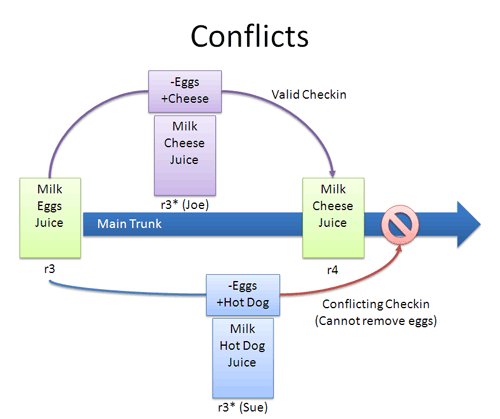
\includegraphics[height=6cm]{vcs_conflict.png}
      
            \end{block}
      
    \end{frame}
    
    \begin{frame}[fragile]{Etiquetes o Tags}
      
            \begin{block}{Etiquetes o Tags}
      
              \begin{itemize}
                \item Podem marcar la revisió per tenir una etiqueta identificativa de la revisió
                
              \end{itemize}

              \centering
              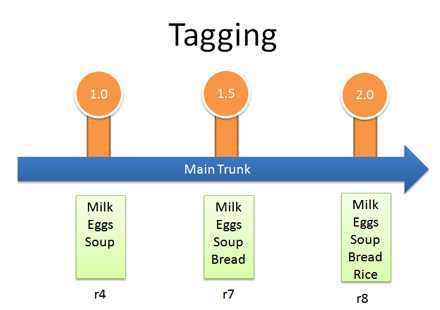
\includegraphics[height=6cm]{tagging.png}
      
            \end{block}
      
    \end{frame}

    \begin{frame}[fragile]{Merge en sistemes distribuïts}
      
            \begin{block}{Merge en sistemes distribuïts}
      
              \begin{itemize}
                \item En sistemes distribuïts es fan unions entre les branques dels desenvolupadors
                
              \end{itemize}

              \centering
              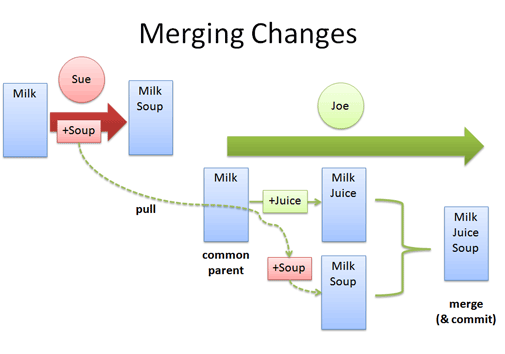
\includegraphics[height=6cm]{distributed_merge.png}
      
            \end{block}
      
    \end{frame}  

    \begin{frame}[fragile]{Organització d'un projecte en sistemes distribuïts}
      
            \begin{block}{Organització d'un projecte en sistemes distribuïts}
      
              \begin{itemize}
                \item Els programadors comproven els canvis en una branca comuna
                \item El responsable revisa els canvis i ho envia a la branca stable
              \end{itemize}

              \centering
              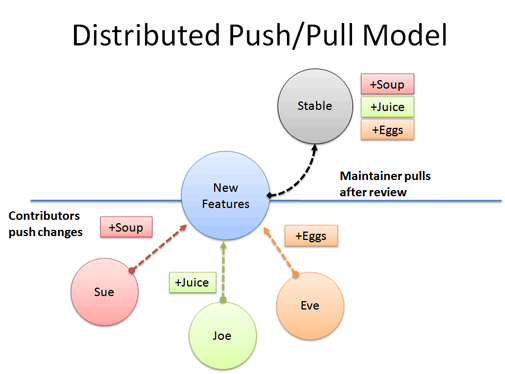
\includegraphics[height=6cm]{distributed_push_pull.png}
      
            \end{block}
      
    \end{frame}  

    \section{Pràctiques}

    \section{Conclusions}
    
    \begin{frame}{Resum}
    
    \end{frame}
    
    \begin{frame}[standout]
      Preguntes?
    \end{frame}

    \begin{frame}{}
      Gràcies per la vostra assistència
    \end{frame}
    
\end{document}
    